%
% FH Technikum Wien
% !TEX encoding = UTF-8 Unicode
%
% Erstellung von Master- und Bachelorarbeiten an der FH Technikum Wien mit Hilfe von LaTeX und der Klasse TWBOOK
%
% Um ein eigenes Dokument zu erstellen, müssen Sie folgendes ergänzen:
% 1) Mit \documentclass[..] einstellen: Master- oder Bachelorarbeit, Studiengang und Sprache
% 2) Mit \newcommand{\FHTWCitationType}.. Zitierstandard festlegen (wird in der Regel vom Studiengang vorgegeben - bitte erfragen)
% 3) Deckblatt, Kurzfassung, etc. ausfüllen
% 4) und die Arbeit schreiben (die verwendeten Literaturquellen in Literatur.bib eintragen)
%
% Getestet mit TeXstudio mit Zeichenkodierung ISO-8859-1 (=ansinew/latin1) und MikTex unter Windows
% Zu beachten ist, dass die Kodierung der Datei mit der Kodierung des paketes inputenc zusammen passt!
% Die Kodierung der Datei twbook.cls MUSS ANSI betragen!
% Bei der Verwendung von UTF8 muss dnicht nur die Kodierung des Dokuments auf UTF8 gestellt sein, sondern auch die des BibTex-Files!
%
% Bugreports und Feedback bitte per E-Mail an latex@technikum-wien.at
%
% Versionen
% *) V0.7: 9.1.2015, RO: Modeline angepasst und verschoben
% *) V0.6: 10.10.2014, RO: Weitere Anpassung an die UK
% *) V0.5: 8.8.2014, WK: Literaturquellen überarbeitet und angepasst
% *) V0.4: 4.8.2014, WK: Initalversion in SVN eingespielt
%
\documentclass[Bachelor,BIF,english]{twbook}
\usepackage[utf8]{inputenc}
\usepackage[T1]{fontenc}

%
% Bitte in der folgenden Zeile den Zitierstandard festlegen
\newcommand{\FHTWCitationType}{IEEE} % IEEE oder HARVARD möglich - wenn Sie zwischen IEEE und HARVARD wechseln, bitte die temorären Dateien (aux, bbl, ...) löschen
%
\ifthenelse{\equal{\FHTWCitationType}{HARVARD}}{\usepackage{harvard}}{\usepackage{bibgerm}}

% Definition Code-Listings Formatierung:
\usepackage[final]{listings}
\lstset{captionpos=b, numberbychapter=false,caption=\lstname,frame=single, numbers=left, stepnumber=1, numbersep=2pt, xleftmargin=15pt, framexleftmargin=15pt, numberstyle=\tiny, tabsize=3, columns=fixed, basicstyle={\fontfamily{pcr}\selectfont\footnotesize}, keywordstyle=\bfseries, commentstyle={\color[gray]{0.33}\itshape}, stringstyle=\color[gray]{0.25}, breaklines, breakatwhitespace, breakautoindent}
\lstloadlanguages{[ANSI]C, C++, [gnu]make, gnuplot, Matlab}

%Formatieren des Quellcodeverzeichnisses
\makeatletter
% Setzen der Bezeichnungen für das Quellcodeverzeichnis/Abkürzungsverzeichnis in Abhängigkeit von der eingestellten Sprache
\providecommand\listacroname{}
\@ifclasswith{twbook}{english}
{%
    \renewcommand\lstlistingname{Code}
    \renewcommand\lstlistlistingname{List of Code}
    \renewcommand\listacroname{List of Abbreviations}
}{%
    \renewcommand\lstlistingname{Quellcode}
    \renewcommand\lstlistlistingname{Quellcodeverzeichnis}
    \renewcommand\listacroname{Abkürzungsverzeichnis}
}
% Wenn die Option listof=entryprefix gewählt wurde, Definition des Entyprefixes für das Quellcodeverzeichnis. Definition des Macros listoflolentryname analog zu listoflofentryname und listoflotentryname der KOMA-Klasse
\@ifclasswith{scrbook}{listof=entryprefix}
{%
    \newcommand\listoflolentryname\lstlistingname
}{%
}
\makeatother
\newcommand{\listofcode}{\phantomsection\lstlistoflistings}

% Die nachfolgenden Pakete stellen sonst nicht benötigte Features zur Verfügung
\usepackage{blindtext}
\usepackage{parskip}

%
% Einträge für Deckblatt, Kurzfassung, etc.
%
\title{A Comparative View of Cross-compiled and Interpreted Cross-Platform Approaches for iOS and Android Mobile Application Development}
\author{Dominik Hack}
\studentnumber{1610257044}
\supervisor{Dipl.-Ing. Dr.techn. Thomas Polzer}
\place{Vienna}
\kurzfassung{kurzfassung}
\schlagworte{Schlagwort1, Schlagwort2, Schlagwort3, Schlagwort4}
\outline{abstract}
\keywords{Keyword1, Keyword2, Keyword3, Keyword4}

\begin{document}

%Festlegungen für den HARVARD-Zitierstandard
\ifthenelse{\equal{\FHTWCitationType}{HARVARD}}{
\bibliographystyle{Harvard_FHTW_MR}%Zitierstandard FH Technikum Wien, Studiengang Mechatronik/Robotik, Version 1.2e
\citationstyle{dcu}%Correct citation-style (Harvardand, ";" between citations, "," between author and year)
\citationmode{abbr}%use "et al." with first citation
\iflanguage{ngerman}{
    %Deutsch Neue Rechtschreibung
    \newcommand{\citepic}[1]{(Quelle: \protect\cite{#1})}%Zitat: Bild
    \newcommand{\citefig}[2]{(Quelle: \protect\cite{#1}, S. #2)}%Zitat: Bild aus Dokument
    \newcommand{\citefigm}[2]{(Quelle: modifiziert "ubernommen aus \protect\cite{#1}, S. #2)}%Zitat: modifiziertes Bild aus Dokument
    \newcommand{\citep}{\citeasnoun}%In-Line Zitiat entweder mit \citep{} oder \citeasnoun{}
    \newcommand{\acessedthrough}{Verf{\"u}gbar unter:}%Für URL-Angabe
    \newcommand{\acessedthroughp}{Verf{\"u}gbar bei:}%Für URL-Angabe (Geschützte Datenbank, Zugriff durch FH)
    \newcommand{\acessedat}{Zugang am}%Für URL-Datum-Angabe
    \newcommand{\singlepage}{S.}%Für Seitenangabe (einzelne Seite)
    \newcommand{\multiplepages}{S.}%Für Seitenangabe (mehrere Seiten)
    \newcommand{\chapternr}{K.}%Für Kapitelangabe
    \renewcommand{\harvardand}{\&}%Harvardand in Zitaten
    \newcommand{\abstractonly}{ausschließlich Abstract}
    \newcommand{\edition}{. Auflage}%Angabe der Auflage
}{
\iflanguage{german}{
    %Deutsch
    \newcommand{\citepic}[1]{(Quelle: \protect\cite{#1})}%Zitat: Bild
    \newcommand{\citefig}[2]{(Quelle: \protect\cite{#1}, S. #2)}%Zitat: Bild aus Dokument
    \newcommand{\citefigm}[2]{(Quelle: modifiziert "ubernommen aus \protect\cite{#1}, S. #2)}%Zitat: modifiziertes Bild aus Dokument
    \newcommand{\citep}{\citeasnoun}%In-Line Zitiat entweder mit \citep{} oder \citeasnoun{}
    \newcommand{\acessedthrough}{Verf{\"u}gbar unter:}%Für URL-Angabe
    \newcommand{\acessedthroughp}{Verf{\"u}gbar bei:}%Für URL-Angabe (Geschützte Datenbank, Zugriff durch FH)
    \newcommand{\acessedat}{Zugang am}%Für URL-Datum-Angabe
    \newcommand{\singlepage}{S.}%Für Seitenangabe (einzelne Seite)
    \newcommand{\multiplepages}{S.}%Für Seitenangabe (mehrere Seiten)
    \newcommand{\chapternr}{K.}%Für Kapitelangabe
    \renewcommand{\harvardand}{\&}%Harvardand in Zitaten
    \newcommand{\abstractonly}{ausschließlich Abstract}
    \newcommand{\edition}{. Auflage}%Angabe der Auflage
}{
    %Englisch
    \newcommand{\citepic}[1]{(Source: \protect\cite{#1})}%Zitat: Bild
    \newcommand{\citefig}[2]{(Source: \protect\cite{#1}, p. #2)}%Zitat: Bild aus Dokument
    \newcommand{\citefigm}[2]{(Source: taken with modification from \protect\cite{#1}, p. #2)}%Zitat: modifiziertes Bild aus Dokument
    \newcommand{\citep}{\citeasnoun}%In-Line Zitiat entweder mit \citep{} oder \citeasnoun{}
    \newcommand{\acessedthrough}{Available at:}%Für URL-Angabe
    \newcommand{\acessedthroughp}{Available through:}%Für URL-Angabe (Geschützte Datenbank, Zugriff durch FH)
    \newcommand{\acessedat}{Accessed}%Für URL-Datum-Angabe
    \newcommand{\singlepage}{p.}%Für Seitenangabe (einzelne Seite)
    \newcommand{\multiplepages}{pp.}%Für Seitenangabe (mehrere Seiten)
    \newcommand{\chapternr}{Ch.}%Für Kapitelangabe
    \renewcommand{\harvardand}{\&}%Harvardand in Zitaten
    \newcommand{\abstractonly}{Abstract only}
    \newcommand{\edition}{~edition}%Edition -> note, that you have to write "edition = {2nd},"!
}}}

\maketitle

\chapter{Introduction}
Almost everyone owns a smartphone these days, according to studies in 2017, 2 billion of these devices were in circulation worldwide \cite[p.~184]{MartinezLecomte2017}. As more and more companies realize the importance of smartphones, so does the demand for mobile applications for their workers or customer's smartphones. As a result, more developers are needed for mobile application development \cite{GaouarBenamarBendimerad2016} \cite{Danielsson_2016}.
However, there is a problem with mobile applications not every one can run on any operating system. According to a study \cite{OSMarketShare} in 2018, 86.8\% of smartphones worldwide use Android and 13.2\% iOS. \cite[p.~5]{Steczko2016}. Theoretically, one would now have to develop a separate application for each supported platform. This was also the go to way for a long time because the first solutions for cross-platform development based only on web development, which led to a lot of lost performance, no way to use hardware features and the only way to access the application was via the browser \cite[p.~626]{6420693} \cite[p.~1]{7934674}.
\\[\baselineskip]
But a lot has changed since then, now there are different approaches to this problem besides developing a web application. Almost every one of these approaches is already based on some mature frameworks that have already been tested by various researchers through several studies. Latif, Lakhrissi, Nfaoui and Es-Sbai published a paper \cite{7479278} in which they summarized all mobile cross platform development approaches and compared them with each other. As a result of their analysis they identified multiple desirable requirements of any cross platform technology. These requirements are: application scalability and maintainability, access to features of device, auto-optimization of resource consumption, security and a development environment that features intelligent auto-completion systems, debuggers, compilers and simulators for all supported platforms. Another paper \cite{7934674} published by the same authors also discusses mobile cross platform development approaches but concentrates on comparing frameworks that are based on these approaches. In the following chapters of this thesis these mobile development approaches will further be explained and the benefits along with the disadvantages of each will be listed.
\\[\baselineskip]
%aprupter Übergang
By implementing a React Native feature set (e.g. scrollable list, screen transition, background process, native module) and analyzing it through performance parameters like CPU and GPU usage, Jesper Söderberg and Erik Johansson, showcase that even tough a native application has still better performance the difference is not very large and therefore can be ignored for most applications \cite{JohanssonSderberg2018}. Marc Armgren compared a Xamarin application with native applications by running user interface, computational and network benchmark tests \cite{Armgren_2015}. He came to the conclusion that applications that have a high value on the user interface or often request data from the network without high computing power requirements can be implemented on Xamarin. In the computational benchmark tests, however, the native applications led Marc Armgren to conclude that Xamarin's cross-compiler was not yet as optimized as the compilers for the native applications \cite{Armgren_2015}. By analyzing, summarizing and comparing the results of studies listed above and more regarding the frameworks Xamarin and React Native, the potential of the interpreted approach and the cross-compiled approach is discussed in the following chapters.
\\[\baselineskip]
In this thesis various noteworthy results of papers, studies and theses (\cite{Danielsson_2016}, \cite{Axelsson2016}, \cite{Hansson_Vidhall_2016}, \cite{MartinezLecomte2018}, \cite{ZubaBernhard2017EdPb}, \cite{WillocxVossaertNaessens2015}, \cite{MartinezLecomte2017}, \cite{Dickson_2013}, \cite{GaouarBenamarBendimerad2016}, \cite{7479278}, \cite{LinckArne2016}, \cite{7934674}) that either experiment with Xamarin or React Native or both will be summarized and their results presented. Besides performance this thesis will also include other criteria like code sharing, documentation and look and feel. If possible, the results of each criteria will contain a discussion comparing Xamarin and React Native with each other. 
\\[\baselineskip]
The following research questions will be the focus of this thesis:
\begin{itemize}
\item Does an application developed in Xamarin perform as well as one developed in React Native and which performs better compared to a native application created in Android or iOS?
\item How much code of an application written using Xamarin or React Native can be shared between Android and iOS?
\item Do the documentations of Xamarin and React Native lack information needed to develop features?
\item Will the look and feel of a native application created in Xamarin or React Native adhere to the OS user interface guidelines?
\end{itemize}

\newpage
\chapter{Mobile Development Approaches}
To this day, lots of companies, if not all, recognized that offering mobile applications on smartphones or other mobile devices to their customers is crucial to have a chance against the competition \cite{7479278}. If a company chooses to provide a mobile application for their customers, they do not want to offer the mobile application to only half of them. However, to reach all customers a company has to develop their mobile application for multiple platforms \cite[p.~5]{Steczko2016}.
\\[\baselineskip]
Nevertheless, without precisely planning the development and maintenance of multiple mobile applications for various platforms the company could invest more money into the development and maintenance than possibly necessary \cite[p.~1]{JohanssonSderberg2018} \cite[p.~8]{Steczko2016} \cite[p.~757]{Ciman2014}. One of the things to consider is what framework should be used for the development of the application. There are lots of frameworks for mobile application development out there and nearly every framework was build by applying one mobile development approach. Each approach has different advantages and disadvantages, therefore it could be the best or worst depending on the situation \cite{6420693} \cite{7934674}. This means in order to minimize costs and thereby increasing the chance of the projects success it is essential to choose a framework with a suitable mobile development approach for the given situation. To assist in finding the most valuable approach for a project, the following sections summarize the most used mobile development approaches. 

\section{Native Approach}
Choosing the native development approach implicates developing the same application separately for each platform it should be available on. Usually the most commonly used platforms on the market, which to this day are Android (insert company) and iOS (insert company), are chosen to be supported \cite[p.~5]{Steczko2016}. As a result, two applications have to be developed one for Android by using the Android-SDK and Java as the programming language, and one for iOS by using the iOS-SDK and Swift as the programming language \cite[p.~5]{LinckArne2016} \cite{AppleGettingStarted}. Even though this leads to the requirement of different skill sets and therefore potentially more developers being necessary for the development of the application, it also leads to applications developed by utilizing the official platform specific frameworks and tools recommended by the publishers of the platforms. 
\\[\baselineskip]
Through using platform specific frameworks and tools, a developer is able to directly communicate with the operating system of the mobile device to get access to features like sensors or cloud services without having to rely on other alternatives, that can potentially decrease performance, cross-platform applications have to use to communicate with the operating system and get access to the above mentioned features \cite[p.~6]{LinckArne2016}.
\\[\baselineskip]
On the downside each application has a different code base thus each code base has to be maintained. This either means that one developer with knowledge of developing on all platforms needs to work on maintenance for all applications or multiple developers with special knowledge regarding one platform work on the maintenance of each particular platform's application \cite[p.~6]{LinckArne2016}.

\section{Cross-Platform Approaches}
The major goal cross-platform approaches try to aim for is only having to develop and maintain one code base for all different platforms. Other important goals are accessing all platform dependent features and to offer the same performance and look and feel a native application does \cite[p.~1]{7479278} \cite[p.~1]{7934674}. To achieve these goals different solutions were developed. These solutions are the following: 
\begin{itemize}
\item Using an interpreter to call native APIs at runtime \cite[p.~3]{7479278} \cite[p.~4-5]{LinckArne2016} \cite[p.~5-6]{Hansson_Vidhall_2016}.
\item Utilizing a cross-compiler to compile non-native code into a native application \cite[p.~3-4]{7479278} \cite[p.~5]{Hansson_Vidhall_2016}.
\item Developing a web application and displaying it via the browser of the mobile device \cite[p.~2]{7479278} \cite[p.~2-3]{LinckArne2016} \cite[p.~4-5]{Hansson_Vidhall_2016}.
\item Wrapping a web application into a native webview-component \cite[p.~2-3]{7479278} \cite[p.~3-4]{LinckArne2016} \cite[p.~5]{Hansson_Vidhall_2016}.
\item Working with Model driven architecture defined by the Object Management Group to create models that will later on be transformed into native source code \cite[p.~4]{7479278} \cite[p.~3]{7934674}.
\end{itemize}
Every approach besides the ones that transform or compile non-native to native code before runtime suffer from performance issues in comparison with native applications. The worse performance arises, as a result of using an additional layer (browser, webview-component, interpreter) to communicate with the features of the device (e.g. camera) \cite[p.~2,~10]{JohanssonSderberg2018} \cite[p.~5-6]{LinckArne2016} \cite[p.~111]{Keist2016}.
\\[\baselineskip]
While there may be multiple solutions, each approach has its own strengths and weaknesses depending on the situation, therefore none is the best for every possible scenario \cite[p.~110]{Keist2016}. The following chapters describe for each approach how the given approach solves the cross-platform problem, what strengths and weaknesses the given approach has and which frameworks or technologies make use of the given approach.

\subsection{Web Approach}
This approach utilizes are the browsers of mobile devices to implement cross platform applications \cite[p.~2]{7934674}. This is possible through the compliance of different browser manufacturers with the HTML standard of the W3C \cite[p.~2]{LinckArne2016}. Therefore by utilizing HTML, CSS, and JavaScript or other web development technologies the developed application can be used on any device that has a browser installed \cite[p.~2]{7934674}.
\\[\baselineskip]
Because the application can be accessed through the browser nothing has to be installed on the mobile device to use it. In addition, due to web applications are hosted on servers, the browser of the mobile device only needs to display data. Even though having to install nothing is an advantage for the users, the distribution of the application is harder since the mobile application stores cannot be used. Furthermore through connection and network issues the performance of web applications is inferior to native applications. Another problem is that web applications have no way to access hardware features like the camera as a result of the application sandboxing \cite[p.~626]{6420693}. Possible technologies that are based on this approach are Jquery mobile, Sencha touch and Boostrap \cite[p.~2]{7934674}.

\subsection{Hybrid Approach}
As in the web approach, an application is also developed using web technologies, only this time the application is executed inside a native container (WebView in Android, UIWebView in iOS). The browser engine renders the HTML content inside of this container so that the container can display it. Additionally, without the sandboxing of the browser, native functionalities can now be retrieved through an abstract JavaScript bridge \cite[p.~626]{6420693} \cite[p.~2]{7479278}. 
\\[\baselineskip]
In addition, through not requiring the browser, the application can now be distributed via the mobile application store. By using web technologies in the development of the application and the browser engine which then processes the content, the user interface can be reused on any platform. Another advantage of this approach is that the native container uses the computing power of the mobile device more than the web approach and thus achieves a better performance than a pure web application \cite[p.~626]{6420693}. However, the performance of such an application can never be as good as that of a native application, because the execution still takes place in a browser engine \cite[p.~2]{7479278}. Additionally, in order to achieve the look and feel of each platform, third-party libraries must be used and most of the time the style of the application should be adapted for each platform \cite[p.~627]{6420693}. Possible technologies that are based on this approach are PhoneGap and Ionic \cite[p.~2]{7934674}.

\subsection{Cross-compiled Approach}
In this approach, as shown in Figure \ref{Fig1}, source code is created by developers using a common programming language and then converted into platform-specific native code (e.g. Java on Android, Objective-C or Swift on iOS) by so-called cross-compilers to be able to communicate with the common back-end (e.g. business logic, data processing, data management) \cite[p.~3]{7479278} \cite[p.~3]{7934674}.
\begin{figure}[!htbp]
\centering
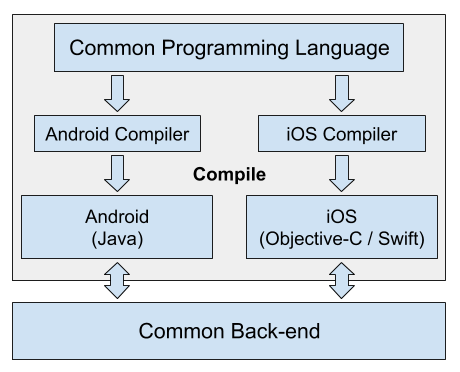
\includegraphics[width=0.5\linewidth]{PICs/Cross-Compiled.png}
\caption{Cross-compiled approach for Android and iOS \cite[p.~3]{7479278}}\label{Fig1}
\end{figure}
As a result of executing the native code compiled by the cross-compiler directly on the mobile device, this approach has almost the same performance as compared to native applications. Through the use of a common programming language and the cross-compilers each hardware feature can be accessed. However, features like camera access, location services, local notifications, etc., cannot be shared between platforms, as each of those features have to be implemented for each supported platform \cite[p.~627]{6420693} \cite[p.~3-4]{7479278}. A possible solution based on this approach is Xamarin \cite[p.~3]{7934674}, this framework will be described in detail in the following chapter and was selected to showcase a comparison between technologies using this approach and the interpreted approach.

\subsection{Model Driven Approach}
The basis for this approach is provided by the Model Driven Architecture of the Object Management Group. The developer creates models with the functionality required for the application. These models are referred to as Computational Independent Models. As shown in Figure \ref{Fig2}, these undergo several transformations to yield platform specific source code at the end that is able to communicate with the common back-end (e.g. business logic, data processing, data management). At first the created models are transformed into Platform Independent Models (PIM). These are then converted to Platform Specific Models (PSM) through the model-to-model transformation. PSMs are, as the name implies, different for each platform and are ultimately transformed into platform-specific source code through a model-to-text transformation. This model-to-text transformation consists normally on a template-based approach \cite[p.~4]{7479278} \cite[p.~3]{7934674}.
\begin{figure}[!htbp]
\centering
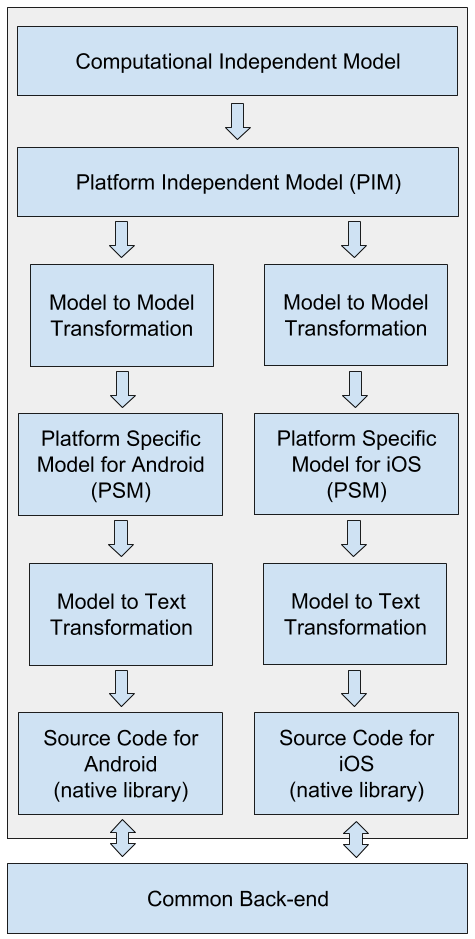
\includegraphics[width=0.5\linewidth]{PICs/MDA.png}
\caption{Transformation from model to source code for Android and iOS \cite[p.~4]{7479278} \cite[p.~3]{7934674}}\label{Fig2}
\end{figure}
\\[\baselineskip]
The problem with this approach is that there is no mature framework based on it. As a result, the full potential of this approach has not yet been demonstrated. Therefore papers regarding the advantages and disadvantages of this approach are rare. However, a prototype framework called MD2 \cite{MD2} already exists, but since it is still relatively young and no official version was released till now, it is still limited \cite[p.~3-4]{7934674}.

\subsection{Interpreted Approach}
In this approach, as shown in Figure \ref{Fig3}, code written in a common language (JavaScript e.g.) 
%is interpreted as native components.
The interpreter is supplied with the application and interprets the code at runtime. In order to have access to hardware functions, the interpreted application communicates with the abstraction layer \cite[p.~3]{7479278} \cite[p.~2]{7934674}.
\begin{figure}[!htbp]
\centering
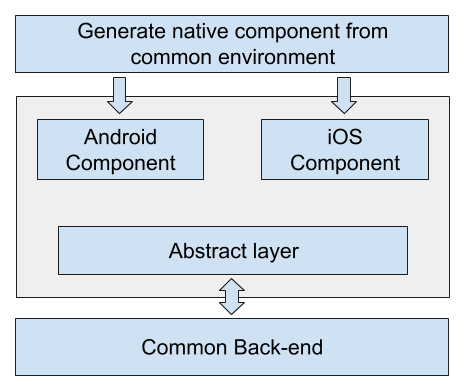
\includegraphics[width=0.5\linewidth]{PICs/Interpreted.png}
\caption{Interpreted approach for Android and iOS \cite[p.~3]{7479278}}\label{Fig3}
\end{figure}
Hardware features can be accessed through special Framework APIs, which simplifies the implementation of a component that requires them. Since native components are generated directly from the common language, the look and feel of the platform on which the application is executed is guaranteed. Despite JavaScript, which is also used in hybrid and web approaches, the interpreter does not require a browser or browser engine, which compared to those approaches leads to an improved performance. However, 
%the same performance can not be achieved as with native applications
because the interpreter needs to interpret the code at runtime \cite[p.~627]{6420693} \cite[p.~3]{7479278}. Technologies using this approach are Appcelerator Titanium and React Native \cite[p.~2]{7934674} \cite[p.~3]{JohanssonSderberg2018}. React Native will be discussed in more detail in the following chapters as it is selected for a comparison of technologies based on this approach with one based on the cross-compiled approach.

\chapter{Selected Frameworks}
Because this paper focuses on presenting a comparison between technologies using either the cross-compiled or interpreted approach, two frameworks had to be chosen. The selected ones are Xamarin and React Native but theoretically there could have been more frameworks selected. However, working with more than one technology per approach would lead to comparing the implementations of the same approach with each other which is not the aim of this thesis. 
\\[\baselineskip]
Though selecting exactly two frameworks does not completely eliminate the possibility of only comparing two implementations with each other that just used a different approach as a solution. Furthermore, if one of these frameworks had a bad implementation, it could yield to far worse results as it another framework using the same approach could achieve. This is why the selected frameworks had to be of high quality, but testing every known cross-platform framework would have exceeded the scope of this thesis, so lots of researching for related work had to be done. 
\\[\baselineskip]
The biggest reasons for selecting Xamarin and React Native were that both support Android and iOS \cite[p.~1]{JohanssonSderberg2018} \cite[p.~12]{ZubaBernhard2017EdPb}, that both still get new features, bug fixes and improvements \cite{XamarinRoadmap} \cite{ReactNativeRoadmap} and a good amount of valuable studies were available to work with (\cite{Hansson_Vidhall_2016}, \cite{MartinezLecomte2018}, \cite{GaouarBenamarBendimerad2016} e.g.).

\section{Xamarin}
With the idea of developing a cross-platform framework that allows writing an application that runs on iOS, Android, Windows and MacOS, the company Xamarin was founded in May 2011. The resulting framework called Xamarin offers the possibility to create a project in which C\# can be used as a programming language to develop a cross-platform application. If hardware features are required that cannot be implemented through the common code, platform specific C\# code can be written into the project of the respective platform in order to be able to implement the feature for this platform. Xamarin was bought by Microsoft in 2016 and is therefore included with every version of Visual Studio \cite[p.~14]{ZubaBernhard2017EdPb} \cite[p.~16]{LinckArne2016}.
\\[\baselineskip]
The basis of Xamarin is the Mono framework, which is an open source implementation of the C\# compiler and the Microsoft .NET framework. In this case, the source code is compiled in bytecode (intermediate language) and then executed by the common language runtime (CLR), also called Mono runtime. In addition, the Mono runtime provides access to an ECMA common language infrastructure (CLI), a just-in-time compiler (JIT) and an ahead-of-time compiler (AOT) \cite[p.~14]{ZubaBernhard2017EdPb}.
\\[\baselineskip]
In order to be able to run the application developed with Xamarin on a mobile device that uses Android, the application must be compiled in bytecode (intermediate language). This is then packed together with the Mono runtime and installed on the device. If the application is now executed the Android runtime (ART) and the Mono runtime run simultaneously. During execution, the Mono Runtime uses its just-in-time compiler to compile the intermediate language to a native assembly. An exchange between the two runtimes is necessary if native functionalities or Java libraries need to be called. The communication between the two runtimes is handled by the Java Native Interface \cite[p.~14-15]{ZubaBernhard2017EdPb} \cite[p.~456]{WillocxVossaertNaessens2015}. Since iOS does not allow generation of code at runtime, the mono-framework's ahead-of-time compiler is used to translate the application's C\# code into native ARM assembler code. This will allow the application to run on iOS\cite[p.~15]{ZubaBernhard2017EdPb} \cite[p.~456]{WillocxVossaertNaessens2015}.
\\[\baselineskip]
When generating a Xamarin project, you can specify whether the project should be created as a Portable Class Library (PCL) or Shared Asset Project (SAP). Both choices allow you to share the common code. The difference is that with PCL, the shared code is packaged into a dynamically-referenced library and then integrated into the various platforms at the runtime of the application. However, with SAP, the common code is already included in the respective projects when the application is built. According to Microsoft, developers should use PCL \cite[p.~16]{ZubaBernhard2017EdPb} \cite[p.~8-9]{Dickson_2013}.
\\[\baselineskip] 
In order to support platform-independent user interfaces with Xamarin, Xamarin.Forms was invented in 2014. When Xamarin.Forms is used, one or more XAML (extensible application markup language) files must be created in which the user interface controls can be defined. During compilation, each XAML file is translated into a BAML (binary application markup language) file, which provides the basis for reusing the user interface across multiple platforms. In addition, each defined user interface control is mapped to the respective native counterpart. However, as a result only those user interface controls can be defined that are also available on all platforms \cite[p.~17-18]{ZubaBernhard2017EdPb}.

\section{React Native}
With the words "learn once, write anywhere" announces Facebook its cross-platform framework, React Native, at the F8 conference in March 2015 \cite[p.~10]{Danielsson_2016} \cite[p.~21]{ZubaBernhard2017EdPb}. With the base of this technology being React, a JavaScript library, React-Native provides the ability to use JavaScript to develop native applications for Android and iOS. In this case, however, no browser is required to render the application, instead the application runs on Android and iOS in a JavaScriptCore VM \cite[p.~10]{Danielsson_2016} \cite[p.~28]{ZubaBernhard2017EdPb}. This, in addition to not needing a WebView container or browser to host the application and transfering the computation of the layout to a thread other than the main thread, makes it possible to develop applications with native responsiveness \cite[p.~10-11]{Danielsson_2016}.
\\[\baselineskip]
Like React Native, React was developed by Facebook, but not in order to enable cross-platform development but to simplify the presentation of complex user interfaces \cite[p.~8]{Danielsson_2016}. On the one hand, this is given by the fact that the complete user interface is divided into so-called components, and on the other hand by the fact that for each imaginable condition of the user interface a so-called state is defined. The user is then presented with a state for each component of the user interface. Depending on the interaction with the user or by receiving data via a web service, these states change \cite[p.~8-9]{Danielsson_2016} \cite[p.~21-27]{ZubaBernhard2017EdPb}. To enable a high-performance reload of the various states, React uses a virtual DOM. This is an abstraction of the real DOM that's only purpose is to assist React by rendering a new virtual DOM, when changes to the data model of a state occur. This result is then compared to the previous virtual DOM and the differences between the two are identified. As a result, only the minimal number of elements in the real DOM have to be reloaded \cite[p.~8-9]{Danielsson_2016}.
\\[\baselineskip]
To enable communication between the native code, the native interface, and the JavaScript code, the Native Bridge was invented. \cite{Hansson_Vidhall_2016} \cite[p.~21-32]{ZubaBernhard2017EdPb}
\begin{figure}[!htbp]
\centering
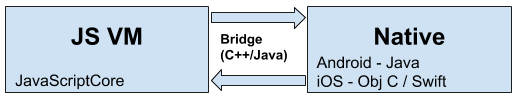
\includegraphics[width=0.75\linewidth]{PICs/Bachelor1_NativeBridge.png}
\caption{Native Bridge for Android and iOS \cite{PicReactNativeBridge} \cite[p.~28]{ZubaBernhard2017EdPb}}\label{Fig4}
\end{figure}

\chapter{Evaluation}
general introduction to criteria and results, why these criteria were chosen, why these studies for the results were chosen, (example: \cite[p.~24]{Danielsson_2016})

\section{Criteria}
introduction of this chapter should give a little start on each criteria, say that each criteria describes the evaluation of the study -> (example: \cite[p.~24]{Danielsson_2016})

\subsection{Performance}
\cite[p.~25-26]{Danielsson_2016} \cite[p.~30]{Axelsson2016} \cite[p.~29-31]{Hansson_Vidhall_2016}

\subsection{Code Sharing}
\cite[p.~31]{Hansson_Vidhall_2016}

\subsection{Documentation}
The purpose of this criteria was to get an idea of how difficult it is to start developing cross-platform applications with either Xamarin or React Native. However, while researching into studies on Xamarin and/or React Native regarding how good or bad the official documentation is, little to no studies were found. The only time authors wrote about the documentation was when they experimented with developing a cross-platform application with either React Native, Xamarin or both. The information contained therein consists mostly of explanations of how the documentation has helped them to solve problems or which information was missing in the official documentation. Some examples of this theses and papers are as follows:
\begin{itemize}
\item Developing a React Native application \cite[p.~16-18]{Danielsson_2016}
\item Developing a geo location and a Bluetooth feature, a shared library and creating native bindings for a Xamarin cross-platform application \cite[p.~10-15]{Dickson_2013} 
\item Porting a HTML5 web application to a React Native cross-platform application and a Xamarin cross-platform application \cite[p.~33-69]{ZubaBernhard2017EdPb}.
\end{itemize}
Considering this led to changing the purpose of this criteria. Before the aim was to compare the official documentations of Xamarin and React Native with each other and finding out if their respective documentation is missing important information. Now the objective is to summarize experiences developers of React Native and Xamarin cross-platform applications had with using the official documentation of either Xamarin or React Native. 

\subsection{Look and Feel}
\cite[p.~18]{GaouarBenamarBendimerad2016}, react native \cite[p.~25]{Danielsson_2016} \cite[p.~31]{Hansson_Vidhall_2016}


\section{Results}
The following chapters showcase and discuss results of studies and experiments regarding the two cross platform mobile development frameworks Xamarin and React Native. When possible, studies were chosen which underwent experiments with both frameworks. However, lots of other noteworthy studies which only underwent experiments with one of the two frameworks are also featured. In this case the results are not comparable, nevertheless not including them would mean ignoring interesting data on the above mentioned criteria. By incorporating these studies, one gains a better picture of Xamarin and React Native regarding performance, code sharing, documentation and look and feel. The studies, which used both frameworks for their experiments, also provided comparisons and discussions of the results. These comparisons and discussions are also summarized in the following chapters.

\subsection{Performance}
xamarin, react native \cite[p.~30-32]{ZubaBernhard2017EdPb}, xamarin \cite{Armgren_2015} \cite{WillocxVossaertNaessens2015}, react native \cite[p.~67-68]{Axelsson2016} \cite[p.~34-43]{Hansson_Vidhall_2016}
\subsection{Code Sharing}
xamarin, react native \cite[p.~71-72]{ZubaBernhard2017EdPb}, xamarin \cite[p.~185]{MartinezLecomte2017}, react native (results\cite[p.~44]{Hansson_Vidhall_2016}) (discussion\cite[p.~53]{Hansson_Vidhall_2016}),

\subsection{Documentation}
At first, the results of the papers concerning the official documentation of React Native are presented, followed by those of Xamarin. At the end other possible sources for information regarding Xamarin and React Native are listed. 
\\[\baselineskip]
The following list includes what experiences William Danielsson had with the documentation of React Native \cite{ReactNativeDoc} while experimenting on developing a replication of an Android application with React Native: 
\begin{itemize}
\item Through following the steps of the documentation's chapter "Getting Started", William Danielsson could set up the development environment for Android and iOS regarding the operating system used on his computer, connect to a physical mobile device, set up a virtual mobile device and create a new project without having a problem \cite[p.~18]{Danielsson_2016}.
\item When trying to implement a feature that captures a photo with the camera of the mobile device multiple errors occurred. One of the problems William Danielsson had to face was that React Native did not support a component for the camera at the time of his experiment. However, Lochlan Wansbrough, a creator of many React Native components, created an open-source camera component. This components repository \cite{ReactNativeCamera} is now part of the official React Native community account \cite{ReactNativeCommunity}. The second problem William Danielsson had was that the documentation of this component only existed for iOS and not for Android. He states that the feature was not implemented for Android because it would have exceeded the scope of his experiment \cite[p.~23-24]{Danielsson_2016}.
\item In order for the same functionalities as in the original application to be offered by the React Native application, it must also be possible to switch from one activity to another. However, as React Native's official documentation did not provide enough information for William Danielsson, he had to access other sources. He solved this problem by consulting the following blog \cite{ReactNativeBlog} \cite[p.~51]{Danielsson_2016}.
\end{itemize}
Jared Dickson's master thesis deals with mobile development with Xamarin, which is why his experiment was based on developing a geo location and a Bluetooth feature, a shared library and creating native bindings for a Xamarin application by using the official documentation of Xamarin \cite{XamarinDoc} as a source for information. However, as he was developing the Bluetooth feature which should have sent messages from one device to another via a Bluetooth connection, he faced the problem that the documentation for implementing a feature that uses a Bluetooth connection on iOS was nonexistent. The experiment was finished without implementing this feature for iOS. However, at the time he was writing his thesis "Core Bluetooth" was released which makes it possible to access the Bluetooth feature on iOS and would have solved his problem, he states \cite[p.~11]{Dickson_2013}.
\\[\baselineskip]
By analyzing a two site long Q\&A Matias Martinez and Sylvain Lecomte tried to find out more about the documentation of Xamarin's error codes. The data for this study was gathered by mining through the questions asked on the Xamarin Forum and on Stack Overflow that contain an error code thrown by the Xamarin framework. On the Xamarin Forum and on Stack Overflow 1121 and 330 questions, respectively, were found, which include one or more Xamarin error codes. 87.5\% of these questions on the Xamarin Forum and 92.3\% of these questions on Stack Overflow have one or more answers. With this information they now plan to analyze these answers and summarize the results to further help developers find a solution for their problem with Xamarin as fast as possible \cite[p.~1,~4]{MartinezLecomte2018}.
\\[\baselineskip]
At last, most authors of these or similar studies, papers or theses have mentioned where they also searched for information during their experiments, these sources will be summarized here. The official documentations of Xamarin and React Native are not the only ways to get detailed information regarding the specific framework. Most developers also use StackOverflow as a source for explanations and code examples \cite{MartinezLecomte2018}. Also when searching for solutions or information regarding a problem with the native code Xamarin and React Native developers can take a look in the official documentations of Android and iOS \cite[p.~11]{Dickson_2013}. More possible sources for information are React's documentation for React Native developers \cite{ReactDoc} and Xamarin Forum for Xamarin developers \cite[p.~51]{Danielsson_2016} \cite{MartinezLecomte2018}.

\subsection{Look and Feel}
xamarin \cite[p.~21]{GaouarBenamarBendimerad2016}, react native (results\cite[p.~29-31]{Danielsson_2016}) (discussion\cite[p.~45]{Danielsson_2016}) (results\cite[p.~44]{Hansson_Vidhall_2016}) (discussion\cite[p.~53-55]{Hansson_Vidhall_2016})


\chapter{Conclusion \& Future Work}








% Hier beginnen die Verzeichnisse.
\clearpage
\ifthenelse{\equal{\FHTWCitationType}{HARVARD}}{}{\bibliographystyle{gerabbrv}}
\bibliography{Literatur}
\clearpage

% Das Abbildungsverzeichnis
\listoffigures
\clearpage

% Das Tabellenverzeichnis
\listoftables
\clearpage

\phantomsection
\addcontentsline{toc}{chapter}{\listacroname}
\chapter*{\listacroname}
\begin{acronym}[XXXXX]
    \acro{iOS}[iOS]{iPhone Operating System}
    \acro{CPU}[CPU]{Central Processing Unit}
    \acro{GPU}[GPU]{Graphics Processing Unit}
    \acro{SDK}[SDK]{Software Development Kit}
    \acro{API}[API]{Application Programming Interface}
    \acro{W3C}[W3C]{World Wide Web Consortium}
    \acro{HTML}[HTML]{Hypertext Markup Language}
    \acro{CSS}[CSS]{Cascading Style Sheets}
    \acro{DOM}[DOM]{Document Object Model}
    \acro{QnA}[Q\&A]{Questions and Answers}
\end{acronym}

\end{document}}